\subsection{RQ4: Which state components create the behavior?}
State removal and flow removal answer different questions. We first pin one state to its neutral score value after every operation: $I=1$, $C=1$, $U=0$, or $T=0$. All weights remain fixed. Removing $T$ removes its state and aging penalty, not elapsed-time integration of the remaining states.
\begin{table}[t]
\centering\small
\caption{State interventions under rapid revision and high interference (eight slots). No retraining; the removed state is pinned to its neutral score value. This experiment differs from the single-flow intervention in Figure~\ref{fig:components}.}\label{tab:ablation}
\begin{tabular}{lrrrr}\toprule
Method & Acc.$\uparrow$ & Stale$\downarrow$ & Ret.$\uparrow$ & Lag$\downarrow$\\\midrule
AME & 75.02 & 0.07 & 88.25 & 15.53\\
No importance & 67.14 & 0.02 & 91.70 & 26.72\\
No consistency & 70.20 & 8.76 & 86.88 & 16.66\\
No usage & 57.91 & 0.11 & 48.51 & 12.85\\
No temporal state & 74.17 & 0.09 & 88.34 & 17.46\\
\bottomrule\end{tabular}

\end{table}

Usage removal produces the largest accuracy and retention loss, while yielding faster first-passage recovery. Consistency removal raises stale error from 0.07\% to 8.76\%. Importance removal increases retention but delays adaptation. These endpoint-specific effects are more informative than treating every component as an interchangeable accuracy improvement.

The second intervention enables only the importance, consistency, or usage \emph{flow}, sweeping its strength over the same seven values. Other states still have their event updates, and $T$ still ages. In rapid/high capacity 8 at strength 1, full evolution achieves SR 87.28\%, AS 0.507, and stale error 0.022\%. Importance-only evolution reaches 75.64\%, 0.260, and 15.11\%, respectively. Consistency-only and usage-only variants retain more stable knowledge but recover more slowly and return more stale answers; these nine endpoint contrasts pass the batch's Holm correction. Single-flow versus full removes two flows simultaneously, so this is evidence for joint behavior, not an orthogonal causal decomposition.
\begin{figure}[!htb]
\centering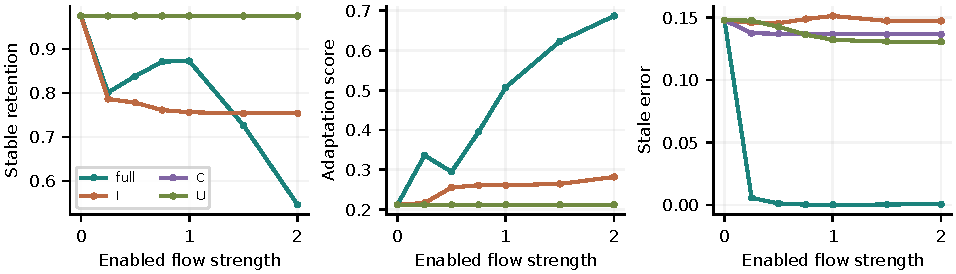
\includegraphics[width=\linewidth]{figures/components.pdf}
\caption{Single-flow interventions under rapid revision, high interference, and eight slots. ``Full'' enables all three flows; I/C/U enable only that flow. Discrete updates remain. All predefined strengths are shown, including unfavorable intermediate values.}\label{fig:components}
\end{figure}
\paragraph{Continuous integration is not the contribution.}
In a separate integration comparison, full evolution achieves 74.80\% accuracy, stable-step Euler integration 74.18\%, and event-only updates 67.26\%. The corresponding stale errors are 0.09\%, 0.09\%, and 14.74\%. These results distinguish event-only behavior from the tested flow but do not establish a unique benefit of exact continuous integration. The event-only variant also removes inter-event $T$ aging, so it is not identical to the zero-strength C1 policy. Adding a query-held context rule reaches 72.49\%, below full evolution; the original controller already receives query-related features.

\paragraph{Resource cost.}
A serial CPU audit on the same 2,344-event schedule measures policy-call time and update counts, separately from trace serialization. State evolution entails $O(K)$ per-event resident work plus a small affine head. No speed or total-memory saving is claimed. Metadata, text, embeddings, and audit logs are outside a simple four-scalar accounting; Appendix~\ref{app:resources} reports the measured audit and its scope.
